% XCircuit output "1.2.tex" for LaTeX input from 1.2.eps
\def\putbox#1#2#3#4{\makebox[0in][l]{\makebox[#1][l]{}\raisebox{\baselineskip}[0in][0in]{\raisebox{#2}[0in][0in]{\scalebox{#3}{#4}}}}}
\def\rightbox#1{\makebox[0in][r]{#1}}
\def\centbox#1{\makebox[0in]{#1}}
\def\topbox#1{\raisebox{-0.60\baselineskip}[0in][0in]{#1}}
\def\midbox#1{\raisebox{-0.20\baselineskip}[0in][0in]{#1}}
   \scalebox{1}{
   \normalsize
   \parbox{1.75521in}{
   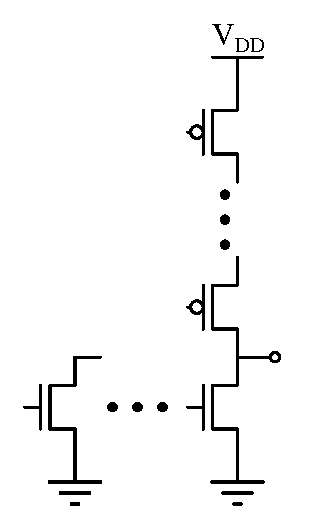
\includegraphics[scale=1]{1.2.eps}\\
   % translate x=496 y=540 scale 0.38
   \putbox{1.47in}{0.62in}{1.20}{1}%
   \putbox{0.39in}{0.62in}{1.20}{1}%
   \putbox{1.56in}{1.29in}{1.20}{2N}%
   \putbox{1.56in}{2.45in}{1.20}{2N}%
   } % close 'parbox'
   } % close 'scalebox'
   \vspace{-\baselineskip} % this is not necessary, but looks better
